%%
%% Beginning of file 'sample.tex'
%%
%% Modified 2015 December
%%
%% This is a sample manuscript marked up using the
%% AASTeX v6.x LaTeX 2e macros.

%% AASTeX is now based on Alexey Vikhlinin's emulateapj.cls 
%% (Copyright 2000-2015).  See the classfile for details.
%%
%% AASTeX requires revtex4-1.cls (http://publish.aps.org/revtex4/) and
%% other external packages (latexsym, graphicx, amssymb, longtable, and epsf).
%% All of these external packages should already be present in the modern TeX 
%% distributions.  If not they can also be obtained at www.ctan.org.

%% The first piece of markup in an AASTeX v6.x document is the \documentclass
%% command. LaTeX will ignore any data that comes before this command. The 
%% documentclass can take an optional argument to modify the output style.
%% The command below calls the preprint style  which will produce a tightly 
%% typeset, one-column, single-spaced document.  It is the default and thus
%% does not need to be explicitly stated.
%%

%% using aastex version 6
\documentclass[twocolumn]{aastex6}
\usepackage{subfigure}
\usepackage{amsmath}

%% The other main article choice is a tightly typeset, two-column article
%% that more closely resembles the final typeset pdf article.
%%
%% \documentclass[twocolumn]{aastex6}
%% 
%% There are other optional arguments one can envoke to allow other 
%% actions. 
%%
% These are the available options:
%   manuscript	: onecolumn, doublespace, 12pt fonts
%   preprint	: onecolumn, single space, 10pt fonts
%   preprint2	: twocolumn, single space, 10pt fonts
%   twocolumn	: a two column article. Probably not needed, but here just in case.
%   onecolumn	: a one column article; default option.
%   twocolappendix: make 2 column appendix
%   onecolappendix: make 1 column appendix is the default. 
%   astrosymb	: Loads Astrosymb font and define \astrocommands. 
%   tighten	: Makes baselineskip slightly smaller
%   times	: uses times font instead of the default
%   linenumbers	: turn on lineno package.
%   trackchanges : required to see the revision mark up and print output
%   numberedappendix: Labels appendix sections A, B, ... This is the default.
%   appendixfloats: Needed. Resets figure and table counters to zero

%% these can be used in any combination, e.g.
%%
%% \documentclass[twocolumn,twocolappendix,linenumbers,trackchanges]{aastex6}

%% If you want to create your own macros, you can do so
%% using \newcommand. Your macros should appear before
%% the \begin{document} command.
%%
\newcommand{\vdag}{(v)^\dagger}
\newcommand\aastex{AAS\TeX}
\newcommand\latex{La\TeX}

%% AASTeX 6.0 supports the ability to suppress the names and affiliations
%% of some authors and displaying them under a "collaboration" banner to
%% minimize the amount of author information that to be printed.  This 
%% should be reserved for articles with an extreme number of authors.
%%
%% Mark up commands to limit the number of authors on the front page.
\AuthorCallLimit=2
%% Will only show Schwarz & Muench since Schwarz and Muench
%% are in the same \author call. 
\fullcollaborationName{The Friends of AASTeX Collaboration}
%% will print the collaboration text after the shortened author list.
%% These commands have to COME BEFORE the \author calls.
%%
%% Note that all of these author will be shown in the published article.
%% This feature is meant to be used prior to acceptance to make the
%% front end of a long author article more manageable.
%% Use \allauthors at the manuscript end to show the full author list.

%% The following command can be used to set the latex table counters.  It
%% is needed in this document because it uses a mix of latex tabular and
%% AASTeX deluxetables.  In general it should not be needed.
%\setcounter{table}{1}

%%%%%%%%%%%%%%%%%%%%%%%%%%%%%%%%%%%%%%%%%%%%%%%%%%%%%%%%%%%%%%%%%%%%%%%%%%%%%%%%
%%
%% The following commented section outlines numerous optional output that
%% can be displayed in the front matter or as running meta-data.
%%
%% You can insert a short comment on the title page using the command below.
%% \slugcomment{Not to appear in Nonlearned J., 45.}
%%
%% If you wish, you may supply running head information, although
%% this information may be modified by the editorial offices.
%%\shorttitle{\aastex sample article}
%%\shortauthors{Schwarz et al.}
%%
%% You can add a light gray and diagonal water-mark to the first page 
%% with this command:
%% \watermark{text}
%% where "text", e.g. DRAFT, is the text to appear.  If the text is 
%% long you can control the water-mark size with:
%% \setwatermarkfontsize{dimension}
%% where dimension is any recognized LaTeX dimension, e.g. pt, in, etc.
%%
%%%%%%%%%%%%%%%%%%%%%%%%%%%%%%%%%%%%%%%%%%%%%%%%%%%%%%%%%%%%%%%%%%%%%%%%%%%%%%%%

%% This is the end of the preamble.  Indicate the beginning of the
%% paper itself with \begin{document}.

\begin{document}

%% LaTeX will automatically break titles if they run longer than
%% one line. However, you may use \\ to force a line break if
%% you desire.

\title{HW 04: Characterizing the Continuum and Emission Lines}

%% Use \author, \affil, plus the \and command to format author and affiliation 
%% information.  If done correctly the peer review system will be able to
%% automatically put the author and affiliation information from the manuscript
%% and save the corresponding author the trouble of entering it by hand.
%%
%% The \affil should be used to document primary affiliations and the
%% \altaffil should be used for secondary affiliations, titles, or email.

%% Authors with the same affiliation can be grouped in a single
%% \author and \affil call.
\author{Bryan Yamashiro\altaffilmark{1}}
\author{Terry Salaga\altaffilmark{2}}
\affil{University of Hawaii at Manoa \\
2500 Campus Road \\
Honolulu, HI 96822}


%% Use the \and command so offset the last author.

%% Notice that each of these authors has alternate affiliations, which
%% are identified by the \altaffilmark after each name.  Specify alternate
%% affiliation information with \altaffiltext, with one command per each
%% affiliation.

\altaffiltext{1}{A cool dude}
\altaffiltext{2}{Another cool dude}


%% From the front matter, we move on to the body of the paper.
%% Sections are demarcated by \section and \subsection, respectively.
%% Observe the use of the LaTeX \label
%% command after the \subsection to give a symbolic KEY to the
%% subsection for cross-referencing in a \ref command.
%% You can use LaTeX's \ref and \label commands to keep track of
%% cross-references to sections, equations, tables, and figures.
%% That way, if you change the order of any elements, LaTeX will
%% automatically renumber them.

%% We recommend that authors also use the natbib \citep
%% and \citet commands to identify citations.  The citations are
%% tied to the reference list via symbolic KEYs. The KEY corresponds
%% to the KEY in the \bibitem in the reference list below. 
\section{Introduction}
Luminous sources produce spectra including both continuous and emission spectra. The continuous spectrum contains light of all wavelengths present, creating a continuum spectrum. Emission lines are emitted by hot rarefied gas at definite wavelengths corresponding to allowed electron transitions and ion capture of free electrons\,\cite{1}. Each stage of ionization of every chemical element has its own individual pattern of emission lines and serves as a unique footprint of the source.
\\
\indent This study examined the spectra of unknown emission sources, and the elemental composition of the unknowns. The spectra in question contains both continuum and emission lines. Another property that will be determined is the temperature of the unknown. Temperature will be determined by an application of Wien's law, provided in equation\,\ref{weins}. Wein's law expresses the relationship of the wavelength at which a black body emits the greatest amount of energy against an inversely proportional absolute temperature\,\cite{1}. The Wein displacement constant, W, is found by differentiating the black body intensity\,(B$_{\lambda}$) with respect to $\lambda$ and setting the derivative equal to zero, yielding a constant of 0.289782\,cm$\cdot$K\,\cite{2}.

\begin{equation}
\lambda_{peak} = \frac{W}{T}
\label{weins}
\end{equation}


%\section{Observations}

\section{Apparatus}


A spectrograph allows for the separation of various wavelengths of light from a radiating source to produce a spectrum\,\cite{1}. The radiating source within the setup included a light that emitted the mystery spectra. Information of the spectra was transmitted through a fiber optics cable that was connected to the spectrograph and the opposing end was focused on the light emitter.





\section{Procedure and Observed Quantities}

The spectra of the unknown source was collected using both the spectrograph for one and four seconds. The one second spectra was chosen to isolate the intense emission line located at the center of the spectra, shown in figure\,\ref{counts}. The four second spectra included other emission lines away from the central wavelengths. Time intervals greater than four seconds maxed out the spectrograph, so no other time interval was used. Three individual runs were carried out for the one second and four second intervals, respectively. The background and dark of the spectrograph were measured before data analysis, and these were conducted with both respective time intervals and runs. The full spectra\,(FS) for both one and four second intervals were then created using the averaged spectra\,($\bar{S}$) and subtracting the average backgrounds\,($\bar{B}$) and average darks\,($\bar{D}$), shown in equation\,\ref{fullspec}.

\begin{equation}
FS_{1,4} = \bar{S} - (\bar{B} - \bar{D}) - \bar{D}
\label{fullspec}
\end{equation}

\begin{figure*}[ht]
  \centering
  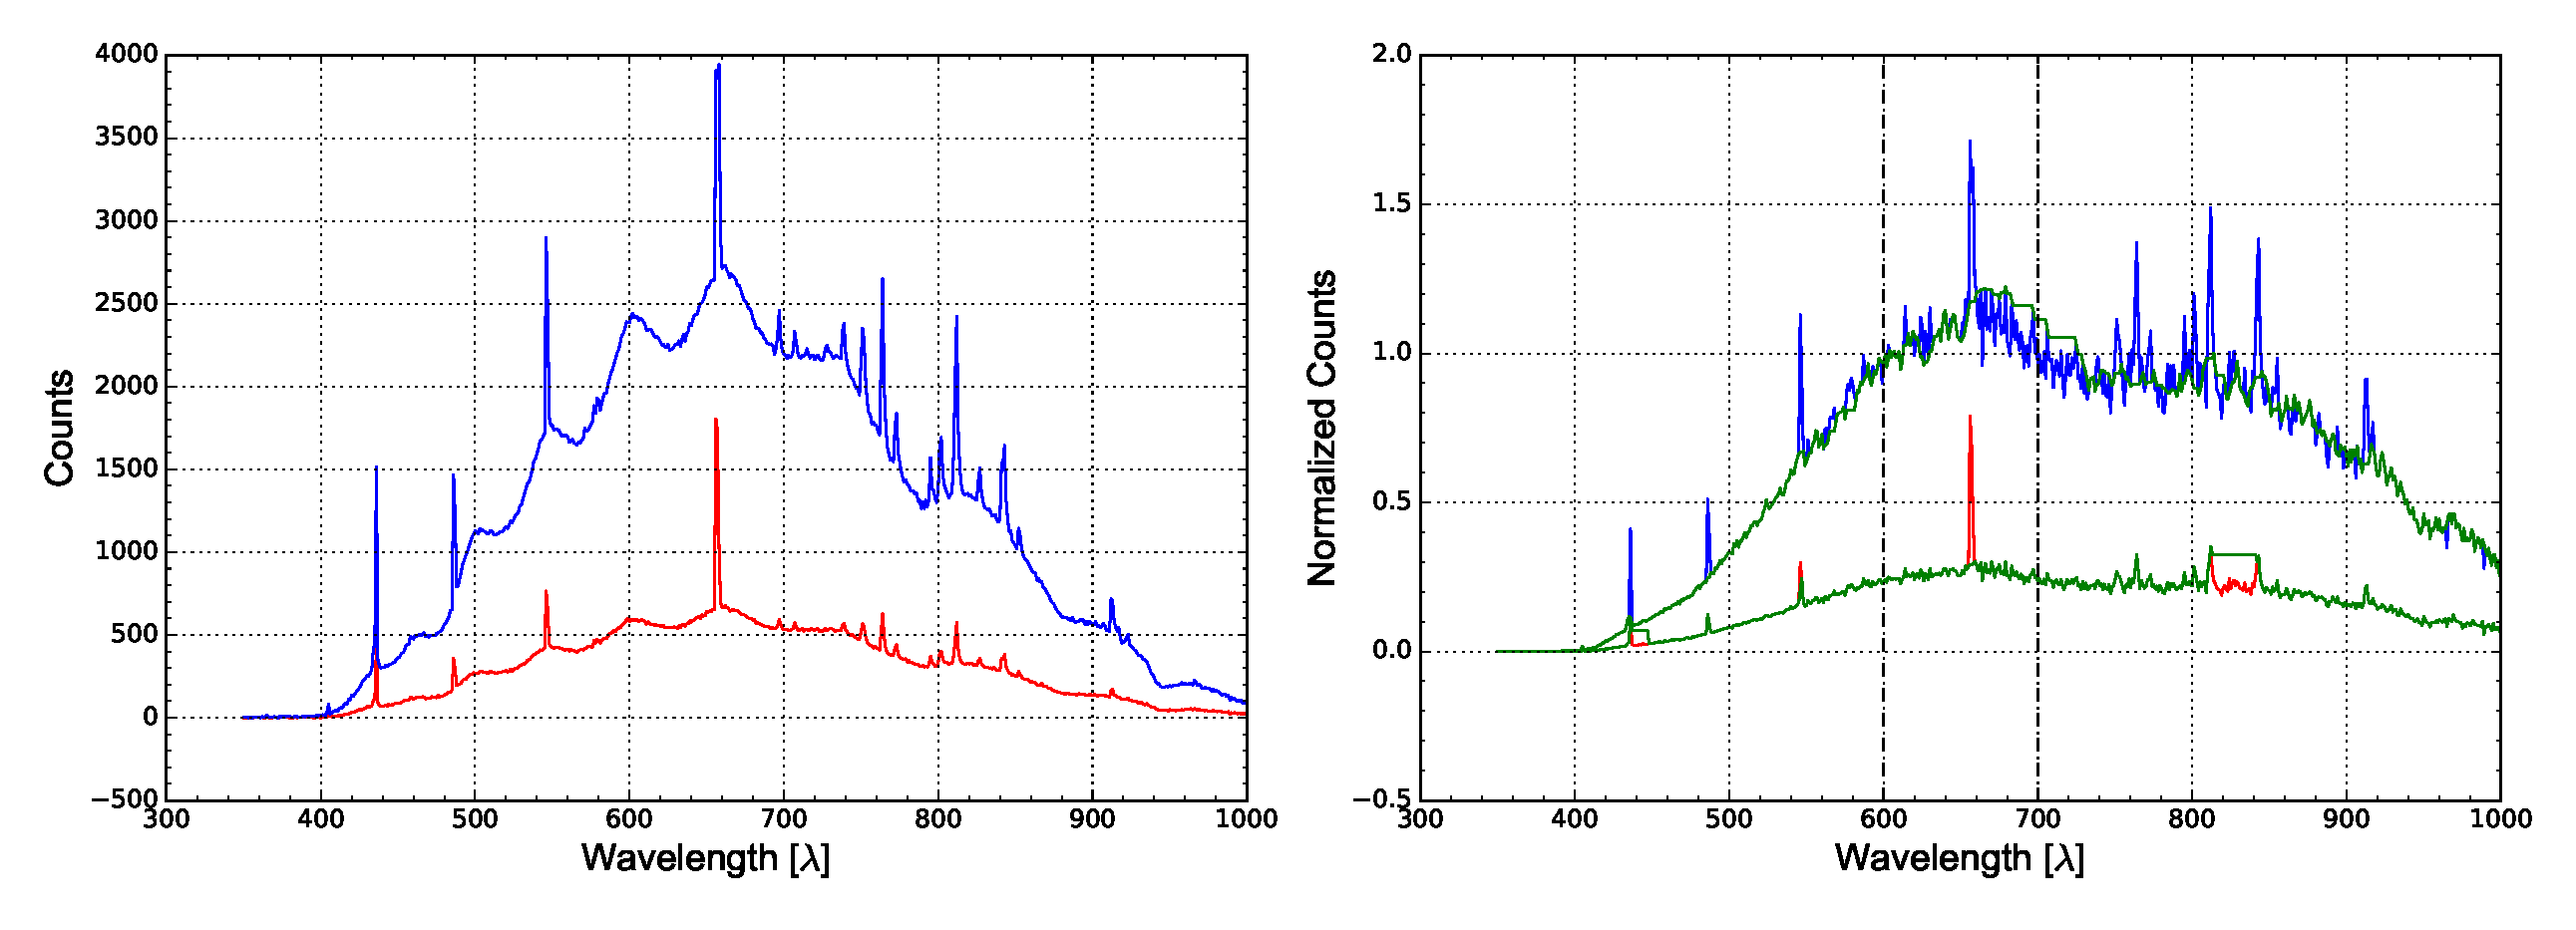
\includegraphics[scale=0.4]{counts.eps}%\quad
  \caption{Full spectra for the mystery emission source with wavelength against counts. The red data represents the 1 second time interval, and conversely, the blue data the 4 second. The left spectra is the raw uncorrected data, whereas the right is the corrected spectrum that includes sensitivity corrections and count normalization. The overlaid green data represents the continuum derived to remove the emission peaks. The black dashed lines represent the region\,(600\,nm - 700\,nm) chosen to deduce the peak wavelength.}
  \label{counts}
\end{figure*}

The raw data gathered from the spectrograph, in figure\,\ref{counts}\,(left), represents the full spectra. To emulate a black body spectrum, a function was introduced to correct the data for the detector sensitivity. A quartz lamp was used to derive the response function and the sensitivity of the detector. The quartz spectrum was measured for the quartz sample using the same techniques as the mystery sample. To obtain the response function, in equation\,\ref{response}, a scaled flux\,(Q$_{SFS}$) was divided by the observed flux\,(Q$_{OF}$) of the quartz spectrum. The scaled flux was derived by initially by deducing the quartz specifications, finding the most wavelength of maximum intensity. This max wavelength was then scaled by the interpolated quartz specifications, producing a scaled flux.

\begin{equation}
R = \frac{Q_{SFS}}{Q_{OF}}
\label{response}
\end{equation}

Figure\,\ref{counts} \,(right) was the generated spectra that included the sensitivity correction of the spectrograph. The continuum represented in green was included primarily to introduce a continuum void of emission lines. The method used to generate the continuum is outlined in equation\,\ref{continuum}. Each wavelength and its corresponding count\,(C$_i$) was compared to next wavelength and count\,(C$_f$). If the difference in count\,($\Delta$C) was higher than an arbitrary specified value\,(x), then the average of the difference\,($\overline{\Delta C}$) was considered to be the count. Contrarily, if $\Delta C$ was lower than x, then C$_i$ was left as the count.


\begin{equation}
C = 
\begin{cases}
C_i ,\quad \Delta C > x \\
\overline{\Delta C},\quad  \Delta C < x 
\end{cases}
\label{continuum}
\end{equation}



\section{Results}

The peak wavelength\,($\lambda_{peak}$), represented in equation\,\ref{peak}, was determined through the corrected spectra and the centroid of the continuum. The centroid of the continuum lies between wavelengths 600\,nm and 700\,cm, so the range was concentrated between those limits. Figure\,ref{counts} clearly illustrates the necessity of the continuum, as equation\,{peak}, would have included the large emission line. The continuum acted as an impetus to more accurately estimate the peak wavelength, compared to the excessive emission flux.

\begin{equation}
\lambda_{peak} = \frac{\sum(\lambda\times flux)}{\sum flux}
\label{peak}
\end{equation}

The uncertainties of the derived wavelengths of the two runs were determined by equation\,\ref{uncert}. It is imperative to note that the uncertainty of the centroid is merely an estimate, but a powerful deduction derived from equation\,\ref{peak}.

\begin{equation}
\sigma_{\lambda_{peak}}^2 = \frac{\sum((\lambda - \lambda_{peak})^2 \times flux)}{\sum flux}
\label{uncert}
\end{equation}

Utilizing equations\,\ref{peak} and\,\ref{uncert}, the peak wavelengths of the continuum were (650.50$\pm$28.63)\,nm and (651.82$\pm$28.85)\,nm for the 1 second and 4 second intervals, respectively. The peak wavelengths were then inserted into the Wein relation, in equation\,\ref{weins}, and the temperatures for the 1 and 4 second intervals were determined to be (4454.76$\pm$196.06)\,K and (4445.74$\pm$196.77)\,K, all provided in table\,\ref{wt}.


\begin{table}[h]
\begin{center}
\caption{The peak wavelength and correlated temperatures for the 1 and 4 second time intervals.}

\begin{tabular}{ c | c | c}
Time Interval & Peak Wavelength & Temperature \\
(s) & (nm) &  (K) \\ \hline \hline
1 & 650.50$\pm$28.63 & 4454.76$\pm$196.06 \\
4 & 651.82$\pm$28.85 & 4445.74$\pm$196.77 \\ 

\end{tabular}
\label{wt}
\end{center}
\end{table}

Finally, the emission lines of the mystery sample were determined using the full corrected spectra. The continuum was subtracted from the full spectra to yield just the emission lines, seen in figure\,\ref{emiss}. All peaks above the specified threshold, above 0.25 normalized counts, was chosen for emission line determination. The threshold of 0.25 normalized counts was used because that value included the most prominent peaks. Every wavelength that resulted in normalized counts over 0.25 were included in table\,\ref{emissions}. If a certain peak contained more than one consecutive wavelengths over the threshold, the values were averaged, specified by the wavelengths ending with 0.5\,nm. Each emission line from the mystery spectrum were overlaid with known gas spectra, provided by the National Institute of Standards and Technology\,(NIST). The nine emission lines from the mystery spectrum corresponded to the known NIST gases hydrogen, mercury, and argon, shown in table\,\ref{emissions}.



\begin{figure*}[ht]
  \centering
  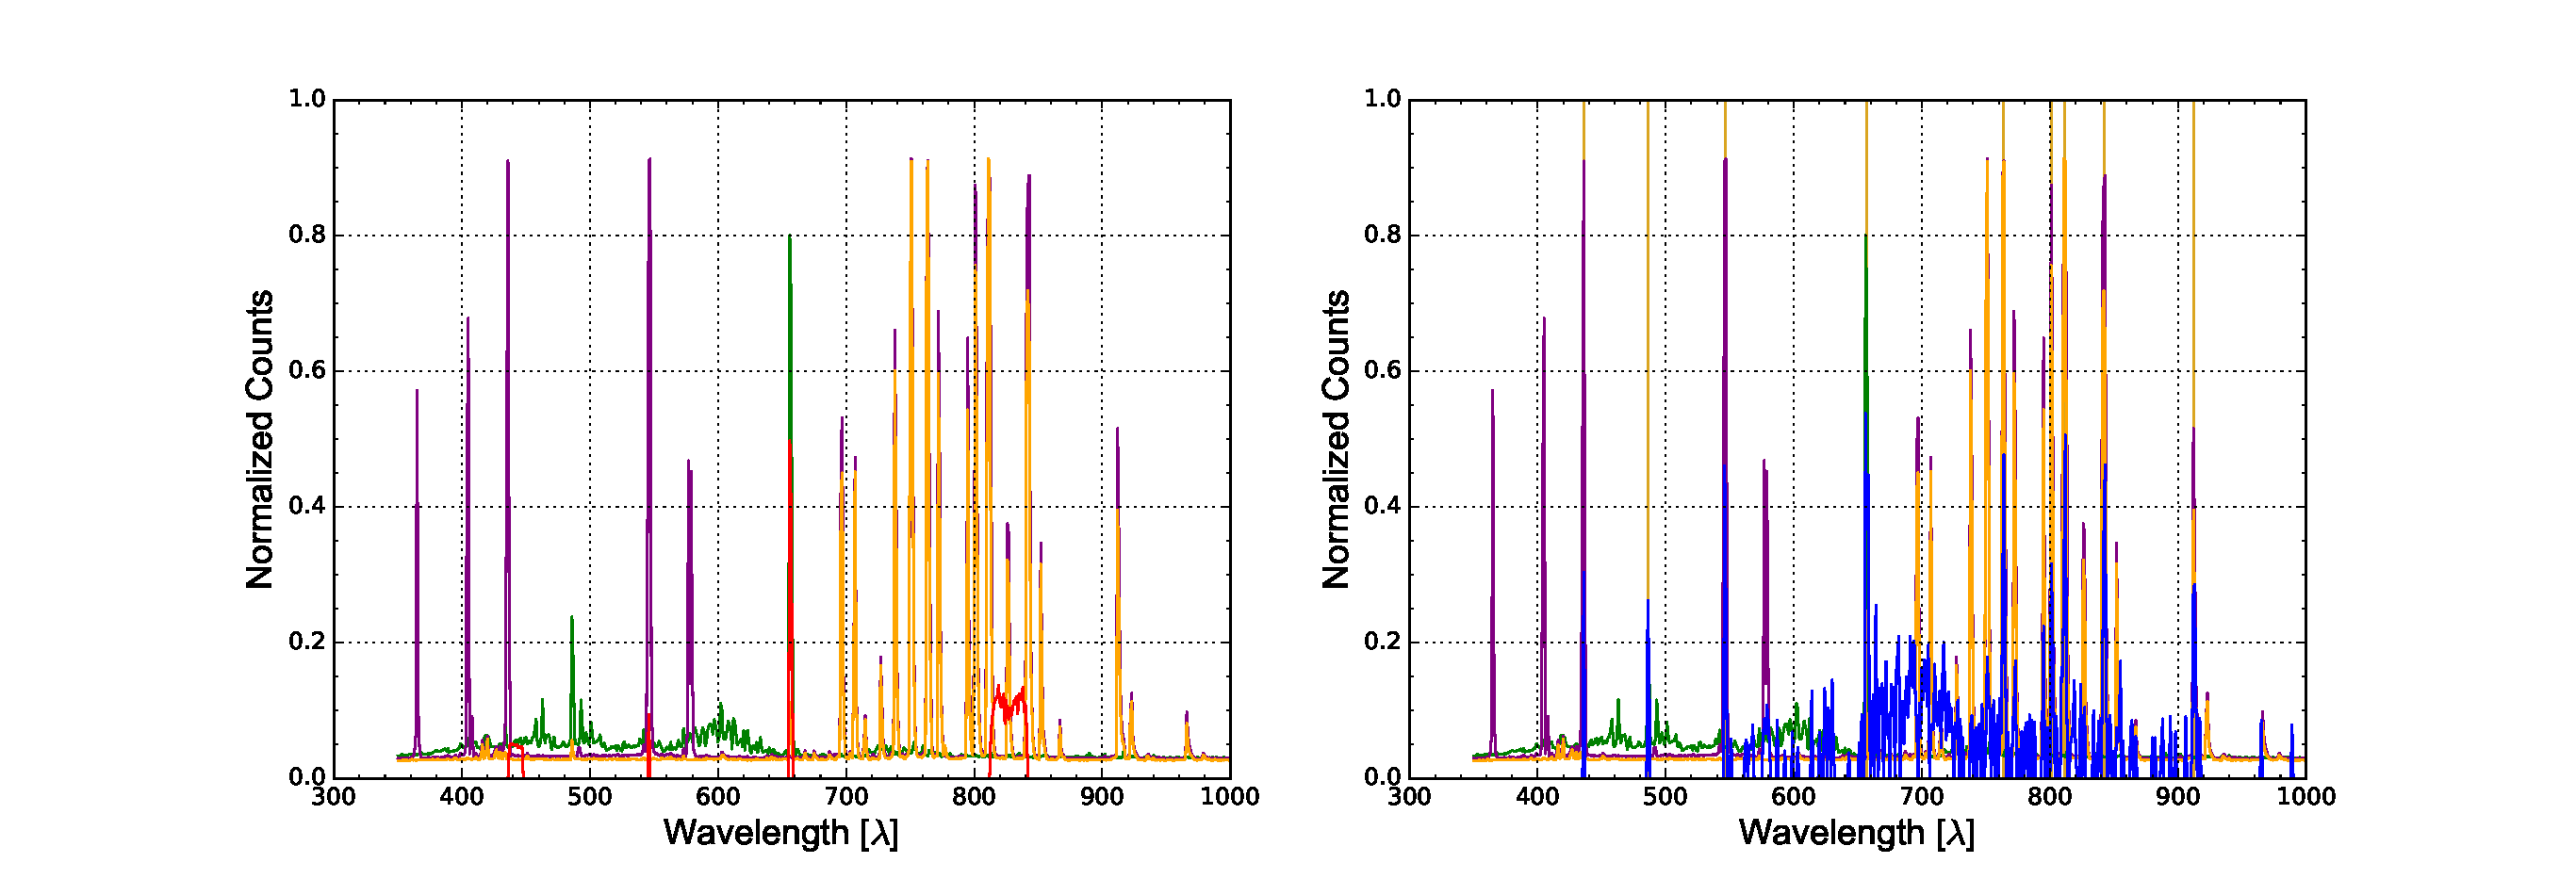
\includegraphics[scale=0.4]{emission.eps}%\quad
  \caption{Emission lines from the full spectra. The plot on the left is the 1 second emission\,(red) and the right plot is the 4 second\,(blue) emission. The hydrogen emission is colored green, and the mercury and argon emission lines are purple and orange, respectively.}
  \label{emiss}
\end{figure*}



\begin{table}[h]
\begin{center}
\caption{Emission lines over a specified normalized count threshold of the full spectra. The emission lines are compared to known values of emission of three known spectra of hydrogen, mercury, and argon. Emission lines on the 4 second emissions above the count threshold are overlaid with goldenrod reference lines to illustrate each of the analyzed wavelengths.}

\begin{tabular}{ c | c | c | c}

Emission Line\,(nm) & Hydrogen & Mercury & Argon \\ \hline \hline
436.0 & - & - & x \\
486.0 & x & - & -  \\ 
546.5 & - & x & -  \\ 
657.0 & x & - & -  \\ 
%664.0 & - & - & -  \\ 
763.5 & - & x & x  \\ 
801.0 & - & x & x  \\ 
811.5 & - & x & x  \\ 
842.5 & - & x & x  \\ 
912.5 & - & x & x  \\ 


\end{tabular}
\label{emissions}
\end{center}
\end{table}

\section{Discussion}

Comparing against known NIST gas emission spectra, the mystery source was a combination of hydrogen, argon, and mercury. After corrections and normalization, the continuum wavelengths of the source were (650.50$\pm$28.63)\,nm and (651.82$\pm$28.85)\,nm for the 1 second and 4 second time intervals, respectively. Wein's law provided the correlating temperatures, which were (4454.76$\pm$196.06)\,K and (4445.74$\pm$196.77)\,K, again for the 1 and 4 second intervals.
\\
\indent Seen in figure\,\ref{emiss}, the continuum showed a large amount of noise at around 700\,nm. Figure\,\ref{counts} shows step-like traits on the continuum, which means that a more precise approach may have resulted in a better continuum. The method of collecting the emission lines was also crude, and Gaussian fits would've yielded more accurate wavelength measurements for each emission line. 


%\acknowledgments



\vspace{5mm}

\begin{thebibliography}{}

\bibitem[Wyatt(1974)]{1}
Wyatt, Stanley P., and James B. Kaler. Principles of Astronomy: A Short Version. Boston: Allyn and Bacon, 1974. Print.

%\bibitem[Herbst(2000)]{1}
%Herbst, W., Maley, J. A., \& Williams, E. C. 2000a, AJ, 120, 349

\bibitem[Aller(1963)]{2}
Aller, Lawrence H. Astrophysics; the Atmospheres of the Sun and Stars. New York: Ronald, 1963. Print.

%\bibitem[Young(2004)]{3}
%Young, Hugh D., and Roger A. Freedman. University Physics. 11th ed. San Francisco: Addison Wesley, 2004. Print.

%\bibitem[Tipler(2004)]{4}
%Tipler, Paul A., and Gene Mosca. Physics for Scientists and Engineers. 5th ed. Vol. 2. New York: W.H. Freeman, 2004. Print. Electricity and Magnetism, Light, Modern Physics.

%\bibitem[Perlmutter(2010)]{5}
%Perlmutter, Saul. "The Plate Scale of a Telescope." Supernova Cosmology Project. Lawrence Berkeley National Lab, Apr. 2010. Web. 27 Sept. 2016.
\end{thebibliography}



%% Appendix material should be preceded with a single \appendix command.
%% There should be a \section command for each appendix. Mark appendix
%% subsections with the same markup you use in the main body of the paper.

%% Each Appendix (indicated with \section) will be lettered A, B, C, etc.
%% The equation counter will reset when it encounters the \appendix
%% command and will number appendix equations (A1), (A2), etc.


%% The reference list follows the main body and any appendices.
%% Use LaTeX's thebibliography environment to mark up your reference list.
%% Note \begin{thebibliography} is followed by an empty set of
%% curly braces.  If you forget this, LaTeX will generate the error
%% "Perhaps a missing \item?".
%%
%% thebibliography produces citations in the text using \bibitem-\cite
%% cross-referencing. Each reference is preceded by a
%% \bibitem command that defines in curly braces the KEY that corresponds
%% to the KEY in the \cite commands (see the first section above).
%% Make sure that you provide a unique KEY for every \bibitem or else the
%% paper will not LaTeX. The square brackets should contain
%% the citation text that LaTeX will insert in
%% place of the \cite commands.

%% We have used macros to produce journal name abbreviations.
%% \aastex provides a number of these for the more frequently-cited journals.
%% See the Author Guide for a list of them.

%% Note that the style of the \bibitem labels (in []) is slightly
%% different from previous examples.  The natbib system solves a host
%% of citation expression problems, but it is necessary to clearly
%% delimit the year from the author name used in the citation.
%% See the natbib documentation for more details and options.


\end{document}

%% End of file `sample.tex'.
